\begin{figure}[!h]
  \begin{center}
    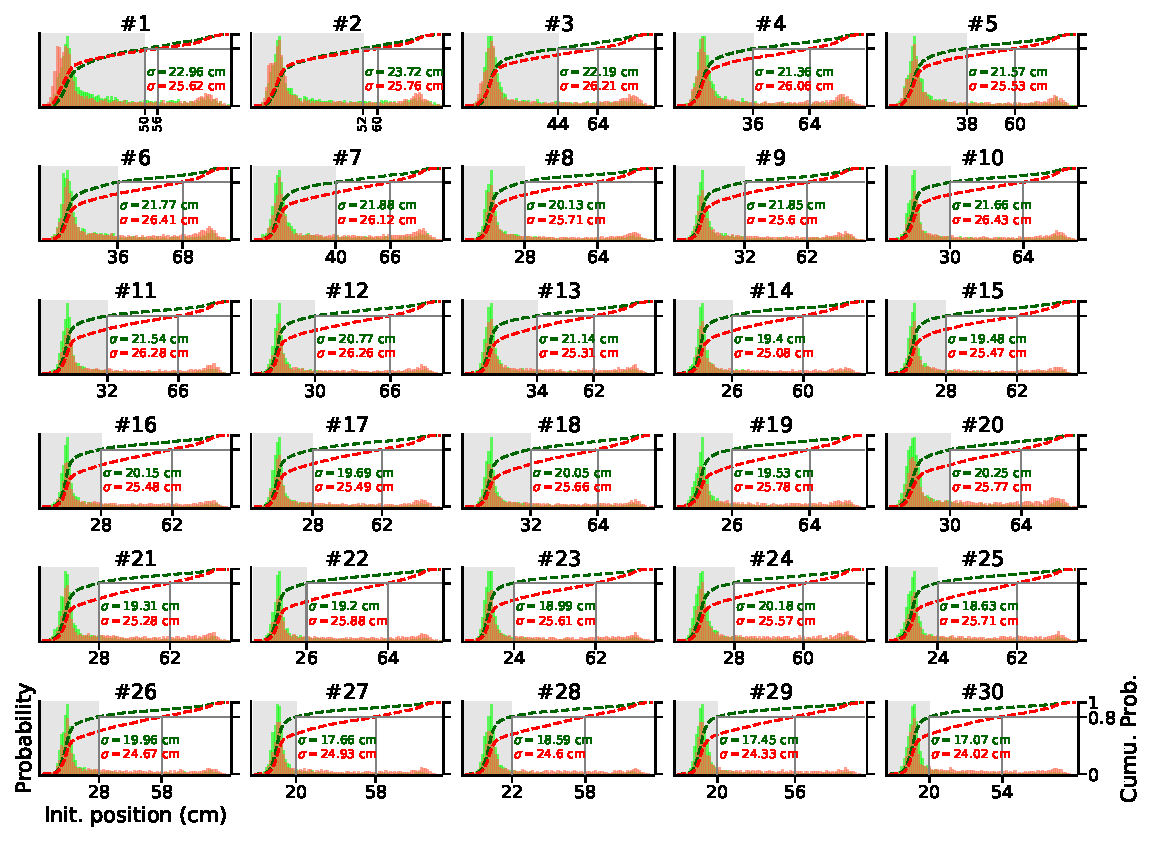
\includegraphics[scale=1]{ch-appendicies/figures/InitPos.pdf}
    \caption[Initial Position Evolution]
    {\textbf{Initial position distributions for correct and error trials diverged progressively during training.}
    Similar to \Autoref{fig:time:CtrlTrd}{e}, each panel shows PDF of the initial position of the animals for correct (green) and error (red) trials, but plotted separately for each training session~(\#1 to~\#30).
    Dashed lines represent cumulative distribution functions (right y-axis).
    For each PDF, $\sigma$ values denote the standard deviation.
    Each PDF included pooled data from all the animals trained in the control condition ($n=54$).
    }
    \label{fig:appendix:initPos}
  \end{center}
\end{figure}